\documentclass[9pt,a4paper]{extarticle}
\usepackage[margin=9.5mm]{geometry}
\usepackage{fontspec}
\usepackage{xcolor}
\usepackage{tabularx}
\usepackage{multicol}
\usepackage{enumitem}
\usepackage{microtype}
\usepackage[hidelinks]{hyperref}
\usepackage{graphicx}
\usepackage{array}
\pagestyle{empty}

\definecolor{navy}{HTML}{102A43}
\definecolor{accent}{HTML}{127A6A}
\definecolor{rule}{HTML}{5B3FA6}
\definecolor{pale}{HTML}{EAF6F3}
\definecolor{ink}{HTML}{243B53}
\definecolor{muted}{HTML}{627D98}
\setmainfont{Avenir Next}
\setsansfont{Avenir Next}
\setlength{\parindent}{0pt}
\setlength{\parskip}{2.0pt}
\setlength{\columnsep}{6mm}
\setlist[itemize]{leftmargin=3.5mm,itemsep=0.4pt,topsep=1.2pt,parsep=0pt}
\renewcommand{\arraystretch}{1.06}

\newcommand{\sect}[1]{\vspace{1pt}{\color{navy}\normalsize\bfseries #1}\par\vspace{0.5pt}{\color{rule}\rule{\linewidth}{0.7pt}}\vspace{0.5pt}}
\newcommand{\metric}[2]{\begin{minipage}[t]{0.47\linewidth}\centering{\color{accent}\large\bfseries #1}\\[-1pt]{\scriptsize\color{muted}#2}\end{minipage}}

\begin{document}

{\raggedright\hyphenpenalty=10000\color{navy}\fontsize{16}{18}\selectfont\bfseries GENCO meets the neutral wire: four-wire dynamic operating envelopes for low-voltage grids}\par
\vspace{2pt}
{\color{accent}\small Extending GENCO to three-phase four-wire low-voltage distribution networks: what breaks, and how a phase-aware extension repairs it}\par
\vspace{2pt}
{\small\textbf{Ander Martinez Alonso\textsuperscript{1,3}, Evgenii Genov\textsuperscript{1}, Rémy Cleenwerck\textsuperscript{1,2}}\quad{\color{muted}\textsuperscript{1}EVERGi, Vrije Universiteit Brussel · \textsuperscript{2}EnSy/Lemcko, Ghent University · \textsuperscript{3}DTU Wind and Energy Systems}}\par
\vspace{3pt}

\colorbox{pale}{\parbox{\dimexpr\linewidth-2\fboxsep\relax}{
\textbf{In brief.} GENCO models the grid as balanced, but European low-voltage networks are three-phase four-wire: every home sits on one phase and the neutral carries the imbalance. On a 200-customer benchmark feeder, envelopes from a balanced model met the four-wire feasibility target in none of the evaluated hours. We found three bottlenecks of GENCO at LV, extended its architecture to an explicit phase-and-neutral network model, and used it as a pre-screen in front of a full four-wire OpenDSS check: six-fold fewer OpenDSS simulations, with zero observed false-safe decisions.
}}

\vspace{3pt}
\begin{multicols}{2}

\sect{The problem}

A \textbf{dynamic operating envelope} (DOE) gives each household a time-varying import and export allowance instead of a fixed connection limit, so that EVs, heat pumps and rooftop PV fit on the existing network.
\begin{itemize}
  \item \textbf{Network:} open-source benchmark ENWL1 (three-phase four-wire, UK), 800\,kVA, 200 single-phase customers, neutral earthed only at the transformer (TT).
  \item \textbf{Households:} Fluvius open data, 2024 quarter-hourly meters; 30\% heat pumps, 30\% EVs, 40\% PV.
  \item \textbf{Limits:} $-$6\%/$+$10\%, i.e.\ 216.2--253.0\,V (UK ESQCR).
  \item \textbf{Check:} an envelope is issued only if OpenDSS finds the network within limits in $\geq$98\% of 200 design scenarios.
\end{itemize}

\sect{Three bottlenecks of GENCO at LV}

The stock model did worse than predicting each bus's average training voltage. We found and fixed:
\begin{itemize}
  \item \textbf{Impedance magnitude:} the edge encoder's layer normalisation suppresses the admittances (10$\times$ admittances change the embedding by 0.2\%). Fix: asinh-scaled features.
  \item \textbf{Physics-loss collapse} at LV scales. Fix: a residual head on a linear power-flow estimate, initialised at zero.
  \item \textbf{Ill-conditioned flows} from voltage differences. Fix: Kirchhoff-current-law flows.
\end{itemize}
Result: voltage error \textbf{1.0e-3\,pu}, 5.4$\times$ below the physics estimate. We also found and fixed two bugs in the GridFM tooling (best-model export; unpinned slack in datakit).

\sect{Operational value}

\begin{center}
\metric{4.81 MWh}{export envelope-hours / household / yr}\hfill
\metric{2.50 MWh}{import envelope-hours / household / yr}
\end{center}
\begin{itemize}
  \item 36 evaluation days of 2024; day-bootstrap intervals 4.35--5.30 (export) and 2.11--2.87\,MWh (import). A fixed allowance valid in every hour would be zero.
  \item Balanced-model envelopes are 2--3$\times$ larger and fail the four-wire check.
\end{itemize}

\columnbreak

\sect{Phase-aware extension as a pre-screen}

The GENCO architecture, extended with a full three-phase four-wire network model (4$\times$4 line impedances, no Kron reduction), corrects a one-step four-wire sweep. On 2,968 evaluation states, under the same final check:

\begin{center}
\metric{35.8\%$\rightarrow$5.8\%}{states sent to OpenDSS}\hfill
\metric{0}{observed false-safe decisions}
\end{center}

Voltage error falls by 91\%. Balanced screens, GENCO included, send 63\% of states to OpenDSS: \textbf{representing the phases is what makes screening useful.}

\sect{Transfer of GENCO representations}
\begin{itemize}
  \item \textbf{Balanced embeddings} in the four-wire model: fallbacks 5.8\%$\rightarrow$11.8\%. They do not carry four-wire information.
  \item \textbf{Official pretrained GENCO} on case118: fine-tuning beat training from scratch by \textbf{+11.4 points} of reference hosting, in 5 of 5 seeds, at 100 labels.
\end{itemize}

\sect{Classical solvers and limitations}
\begin{itemize}
  \item An iterated four-wire sweep remains the accuracy leader (about 80$\times$ more accurate). The learned screen's value is six-fold fewer OpenDSS simulations.
  \item A design-set check, not a certificate of future safety. Not checked: partial uptake, undervoltage during export, neutral current, voltage unbalance. One benchmark feeder.
\end{itemize}

\sect{Open science}
\begin{itemize}
  \item Public inputs (ENWL1, Fluvius open data); pre-registered core evaluation, frozen protocols, disclosed amendments and incidents.
  \item 84 tests; \texttt{reproduce\_check.py} regenerates every headline result byte for byte; one-minute public demo.
\end{itemize}

\textbf{Outlook:} LV envelopes sum to the flexibility a DSO offers upstream; one model across LV, MV and HV needs the three changes identified here.

\end{multicols}

\vspace{1pt}
\begin{center}
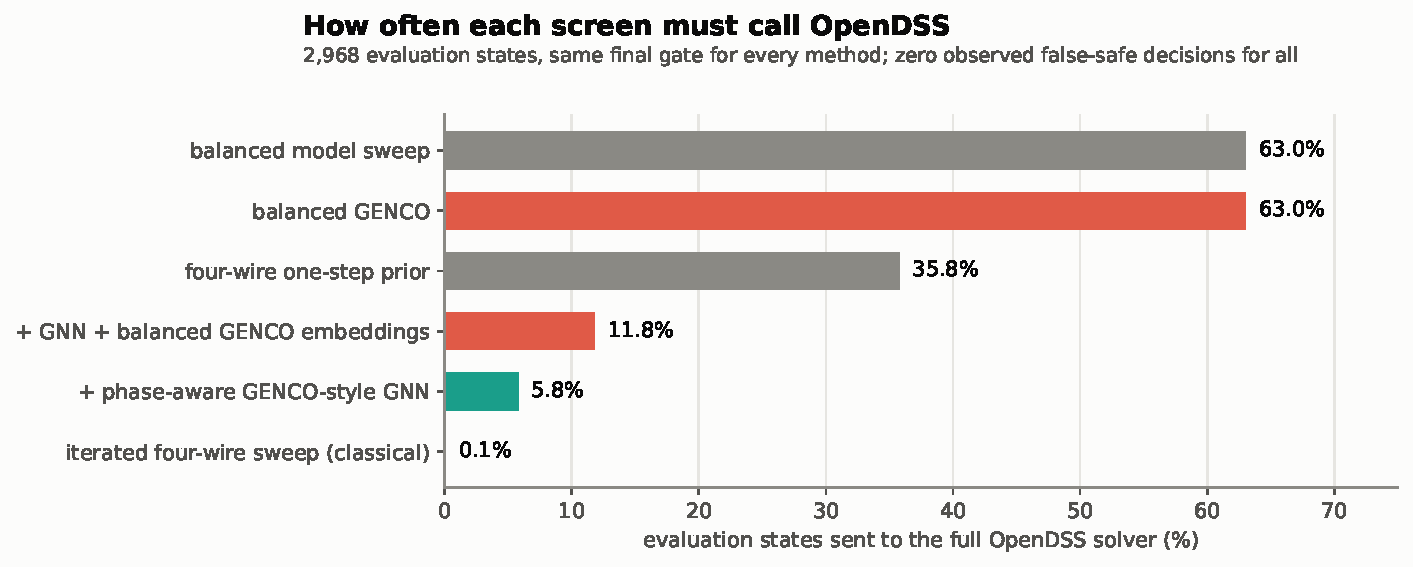
\includegraphics[width=0.66\linewidth]{../figures/fig4a_fallback.pdf}\\[-1pt]
{\scriptsize\color{muted}Share of 2,968 evaluation states each screen sends to OpenDSS, all under the same final check; none made a false-safe decision.}
\end{center}

\vfill
{\footnotesize\color{muted}github.com/ujohn33/genco-dynamic-envelopes · ander.martinez.alonso@vub.be \hfill GridFM GENCO Challenge 2026}

\end{document}
